Energy price prediction is a cumbersome task to handle because of the highly volatile nature and the plethora of factors that influence the energy price. In this section we will show the factors that influence the price by analysing relevant data that will later become input in our ANN. Not to surprisingly the most important factor in any market is demand and this greatly influences the price "REFERENCE". But also time of day, day of the week, wind speed and temperature (which are the quantifiable factors) play a big role and sociocultural influences affects the price aswell. This section will show the connection between energy price and some of the influential factors.

\subsection{Demand}
Demand is directly connected to the energy prices which comes as no suprise since every market is driven by demand. Since demand is relative to the present time we are not able to use it directly as an input factor in the artificial neural network(ANN). We have to compute the demand and this is why we need to know what impacts the demand. As mentioned in related work we have seen a function that calculates the demand based on CDD(Cooling degree days), HDD(Heating degree days), ELD(Humidity), V$_w$ (Wind speed), M$_s$ (Sunshine), M$_r$ (Rainfall) \cite{19}. Based on these factors we will model the ANN to take these factors as inputs. This will be done as either direct input or as a seperate neural network for demand and feed that directly (as input) into the energy price ANN.

\begin{figure}[!ht]
\centering
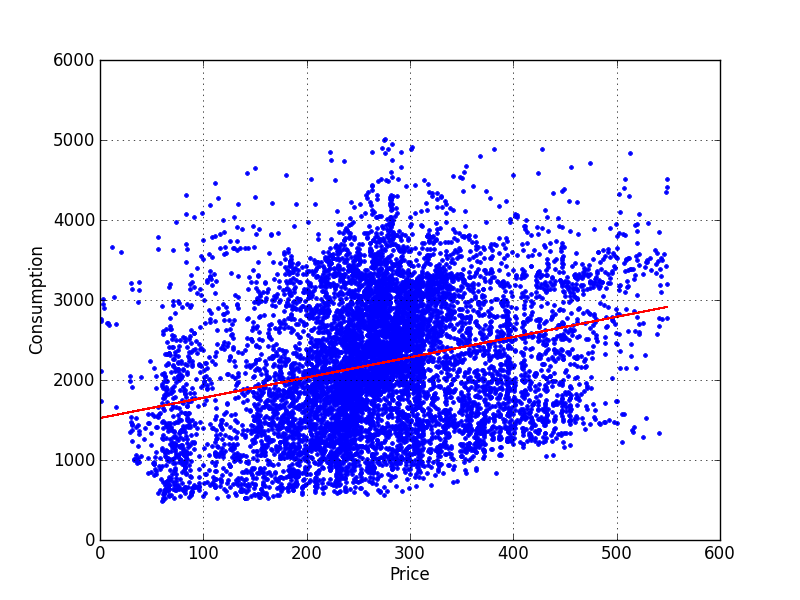
\includegraphics[width=0.8\textwidth ,natwidth=410,natheight=237]{billeder/energy_price_plots/consump_price.png}
\caption{Demand and price plot.}
\label{fig:consump_price}
\end{figure}

In figure ~\ref{fig:consump_price} we see the connection between energy price and the demand. The model shows us that if the demand rises the price on the energy rises aswell. This is a common tendency in a market where there isn't endless supply. Since the price is heavily influenced by demand and demand is a relative factor the same calculations are also done by the powerplants because they need to know how much power to produce in a certain timeframe. We want to imitate this forecast and predict our own demand based on the aforementioned parameters. This is key to how accurate we will be able to predict the price. In other words: A good prediction of the demand will give us a good prediction of the price.

\begin{figure}[!ht]
\centering
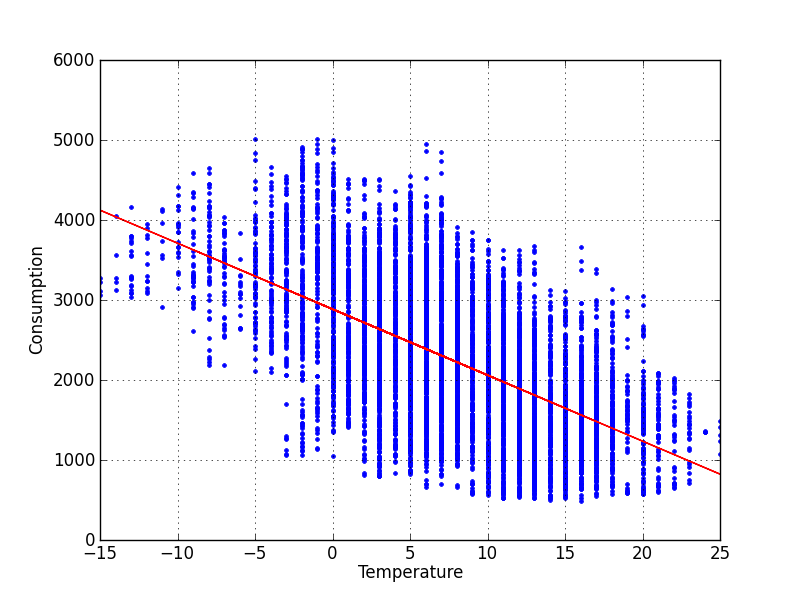
\includegraphics[width=0.8\textwidth ,natwidth=410,natheight=237]{billeder/energy_price_plots/consump_temp.png}
\caption{Demand and temperature plot.}
\label{fig:consump_temp}
\end{figure}


In figure ~\ref{fig:consump_temp} we see the connection between demand and temperature. The temperature itself has an influence when it is very cold or very warm. This connection is expressed as CDD and HDD. In figure ~\ref{fig:consump_temp} we see that if temperature decreases the demand will go up. This is presumably because the people of Denmark use a lot of energy on heating our homes and lighting in the winter time. In \cite{19} they also describe CDD which indicates the need for cooling. In Denmark it is limited how high the temperature goes and how often we actually need to cool our homes.

\subsection{Price}
We present some of the influences on the price in this section and argue why these parameters has an impact on the price. We also account for the time perspective of the price and show the non-linear nature of energy prices. Since we just talked about demand and the influence on price we will here be focusing on the other impacting factors in the prediction of energy prices.

\begin{figure}[!ht]
\centering
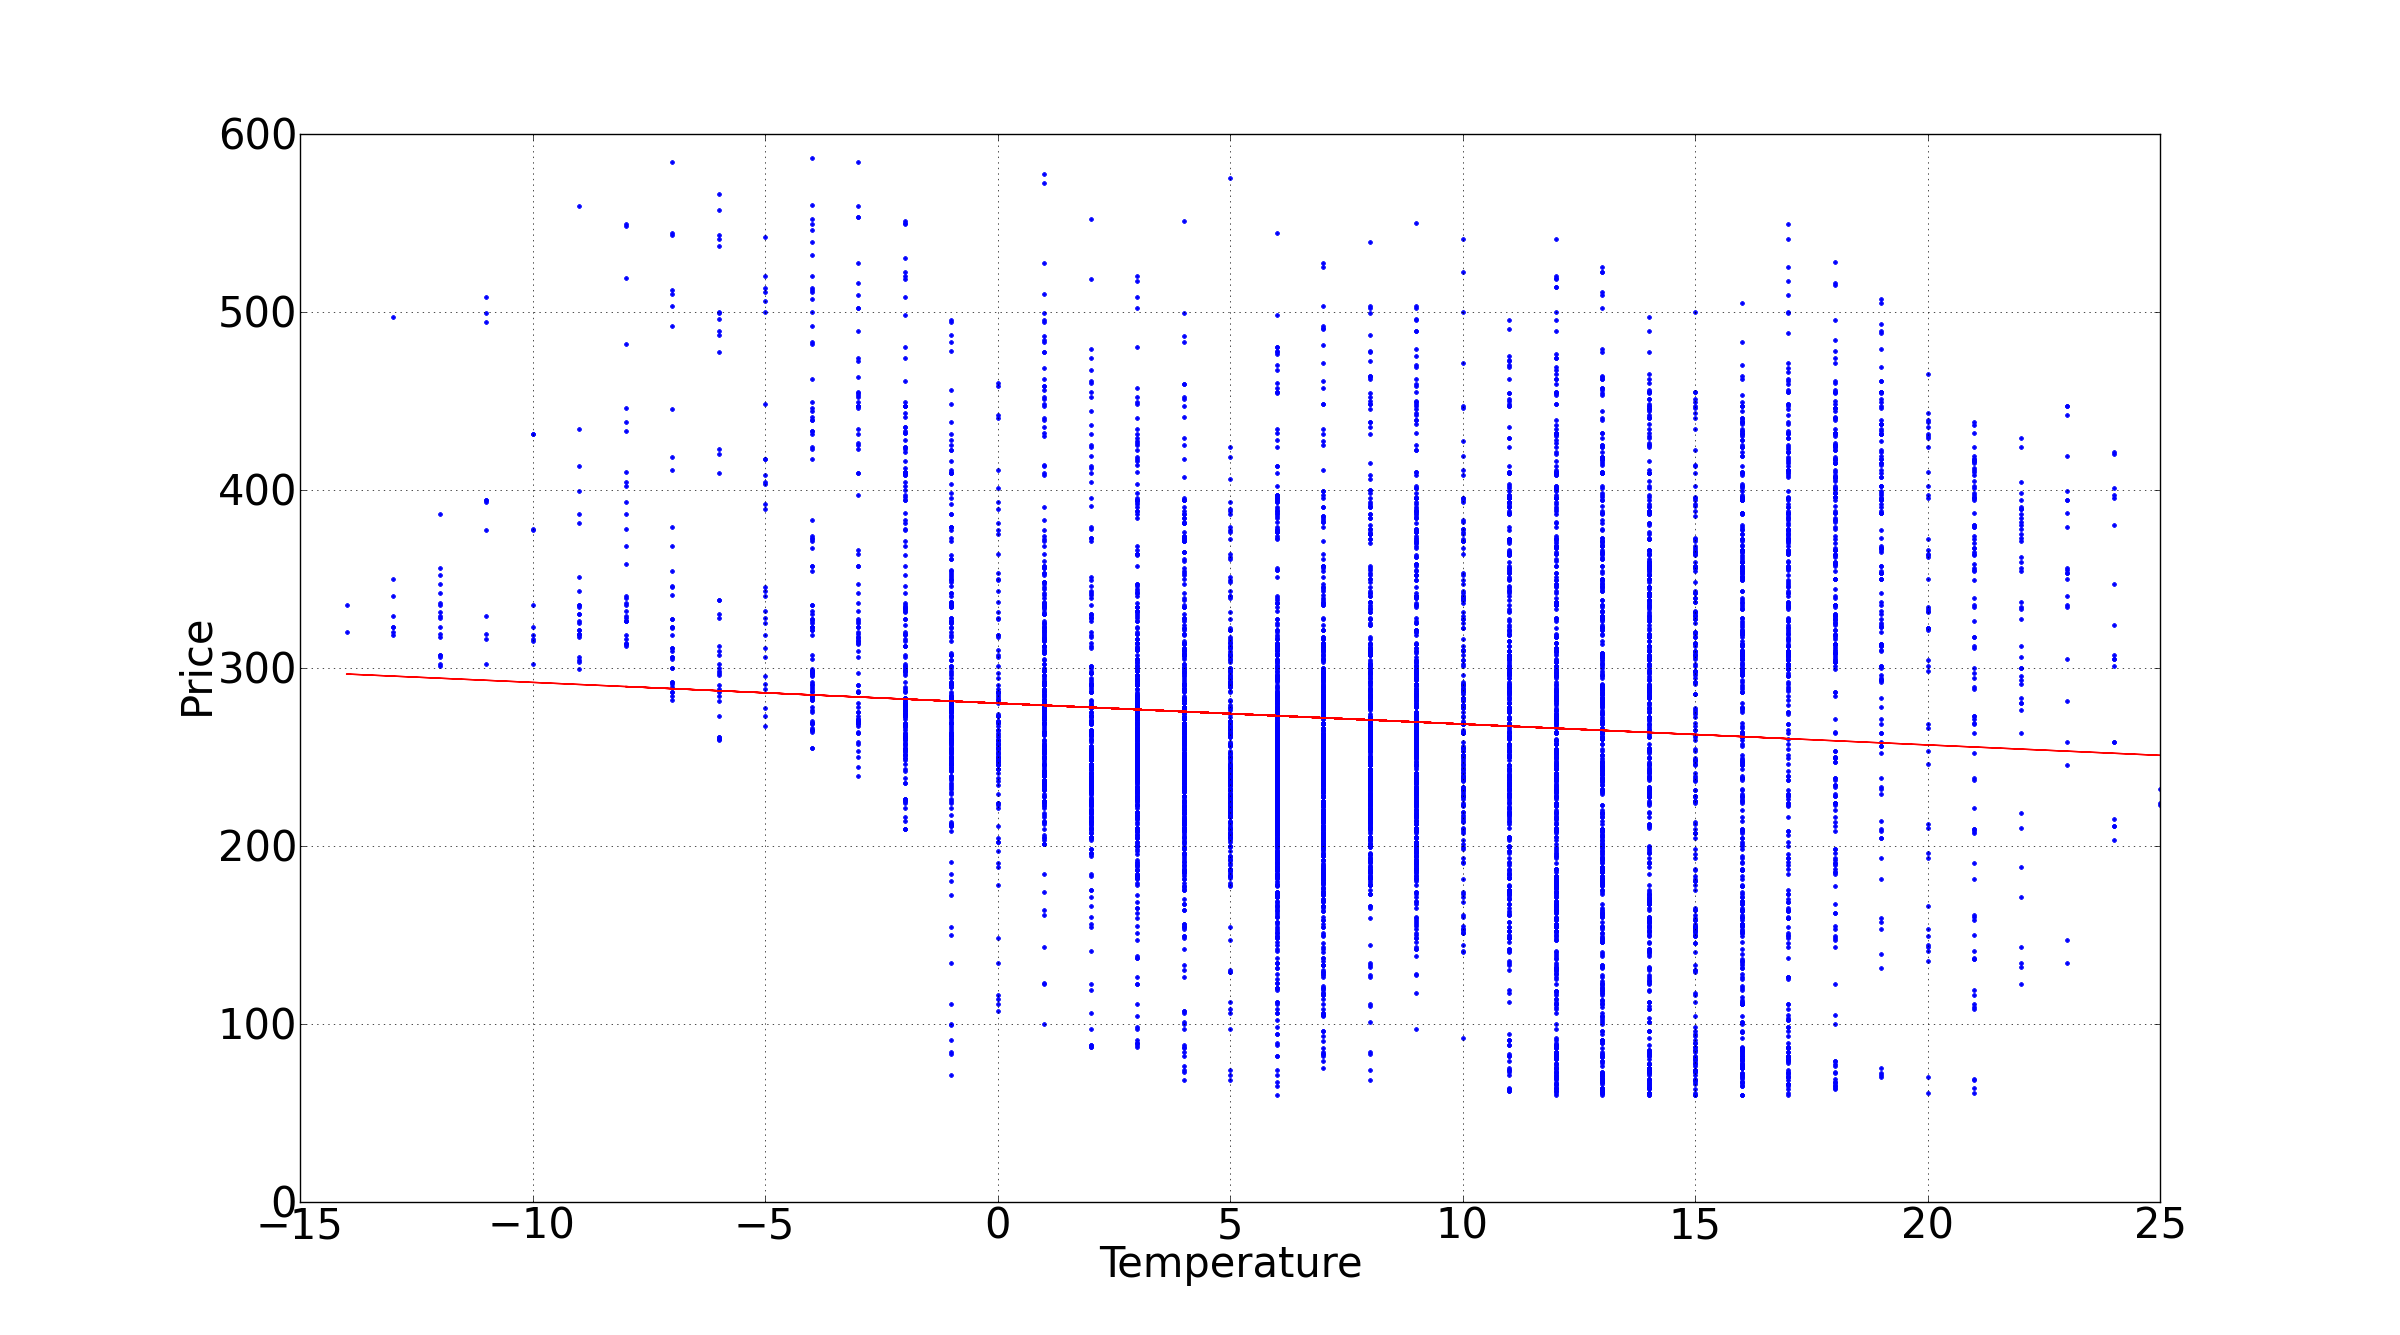
\includegraphics[width=0.8\textwidth ,natwidth=410,natheight=237]{billeder/energy_price_plots/price_temp.png}
\caption{Price and temperature plot.}
\label{fig:price_temp}
\end{figure}

In figure ~\ref{fig:price_temp} we see how the price decreases as the temperature rises. This is due to the same factors as explained in the demand and temperature plot graph. Temperature impacts the demand which impacts the production of energy. If the demand thus the production is high then the price will automatically rise aswell.

\begin{figure}[!ht]
\centering
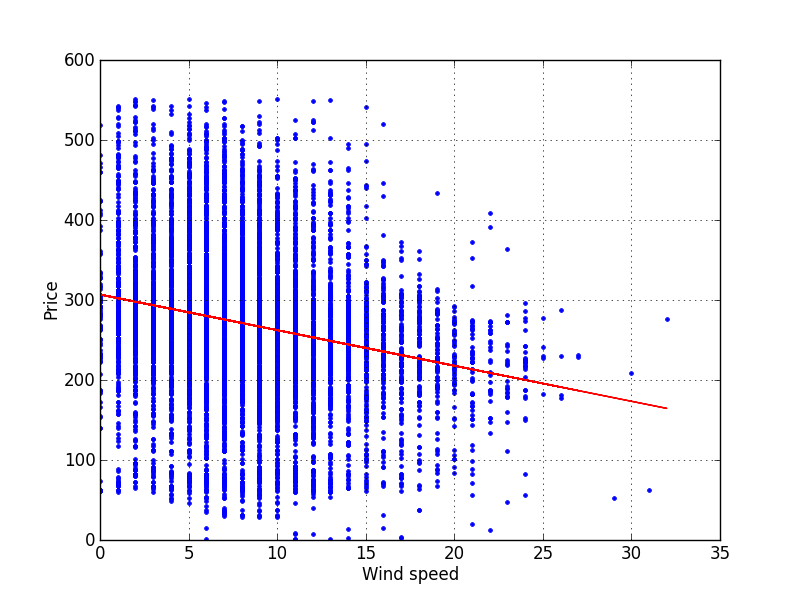
\includegraphics[width=0.8\textwidth ,natwidth=410,natheight=237]{billeder/energy_price_plots/price_wind.png}
\caption{Price and wind plot.}
\label{fig:price_wind}
\end{figure}

In figure ~\ref{fig:price_wind} we see how the wind impacts the price. If the wind speed increases the energy price decreases. This is because the wind power production will allow for a bigger output on the general power production. When the production is high and the demand is moderate the price will decrease to get demand up since we cannot store energy for later use. Also wind power production produces nearly "free" energy when the windmill park is up and running.

\begin{figure}[!ht]
\centering
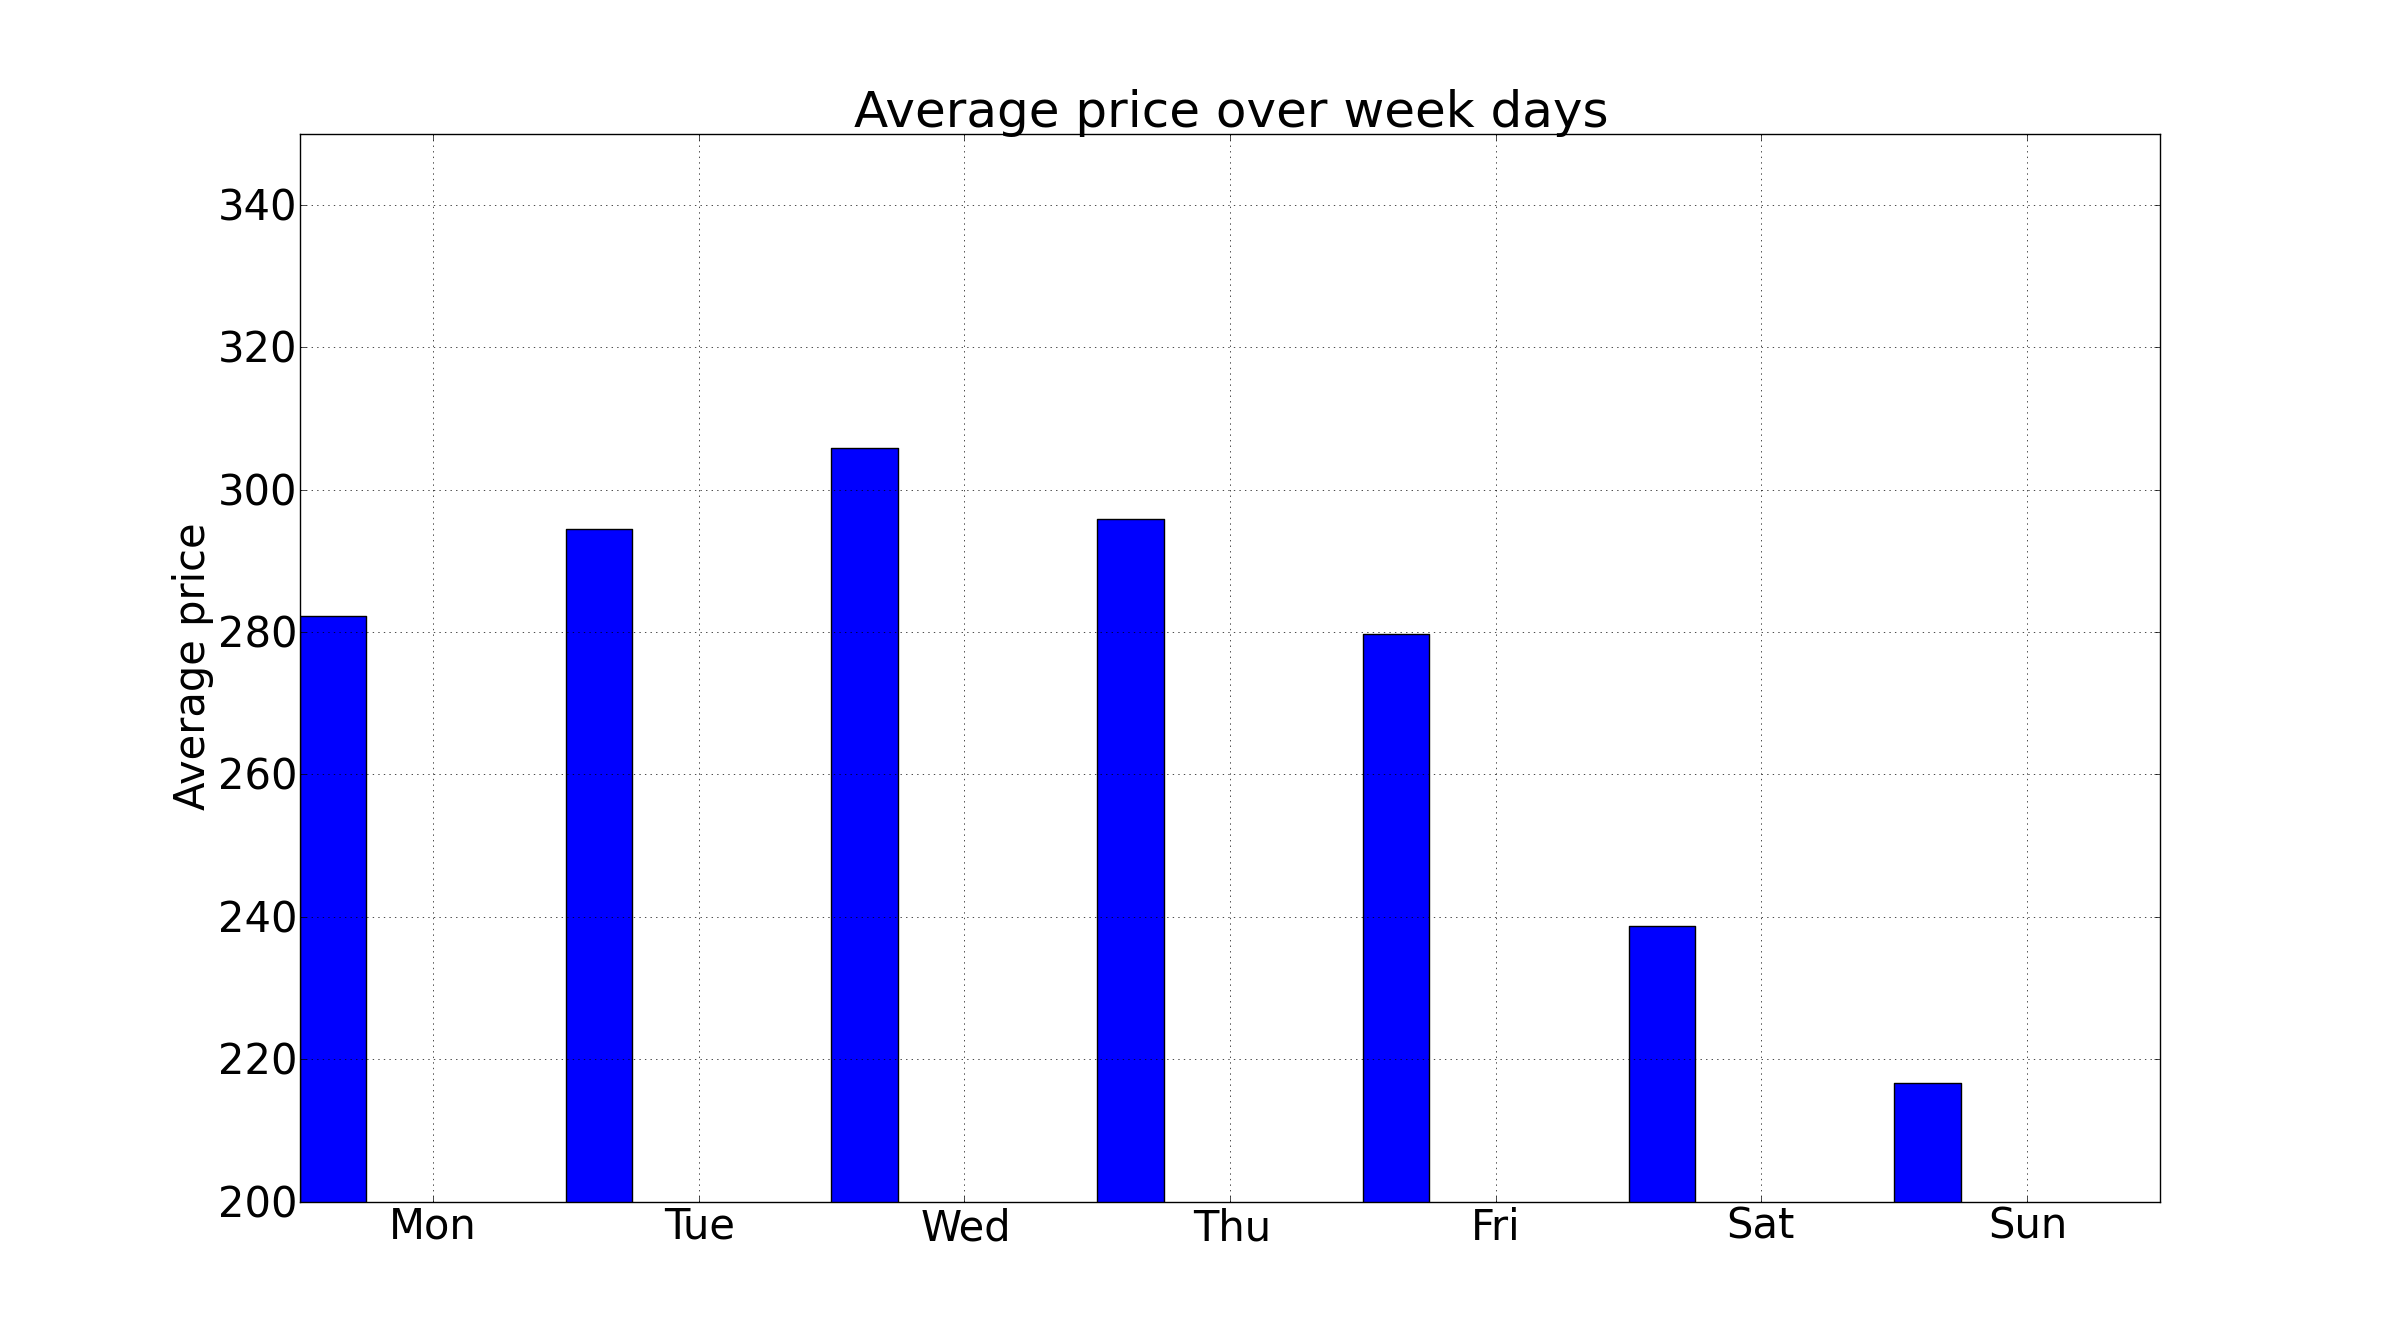
\includegraphics[width=0.8\textwidth ,natwidth=410,natheight=237]{billeder/energy_price_plots/Average_price_over_weekdays.png}
\caption{Price dispersion over weekdays}
\label{fig:price_over_weekdays}
\end{figure}

Figure ~\ref{fig:price_over_weekdays} shows us how the trend of the price varies over the different days in a week. The most noticeable here is how the price is decreasing in the weekend (saturday and sunday) and are somewhat steady for the weekdays. We are looking at two options for our neural network. One is to make a prediction for whole days at a time which are good for days with incomplete information and the other is to predict the hourly price which requires specific data for the given hour. In the daily prediction proposal we will want to distinquish between weekdays and weekends. We will also have to look at seperating saturday and sunday since they show a substantial difference in price per day.

\begin{figure}[!ht]
\centering
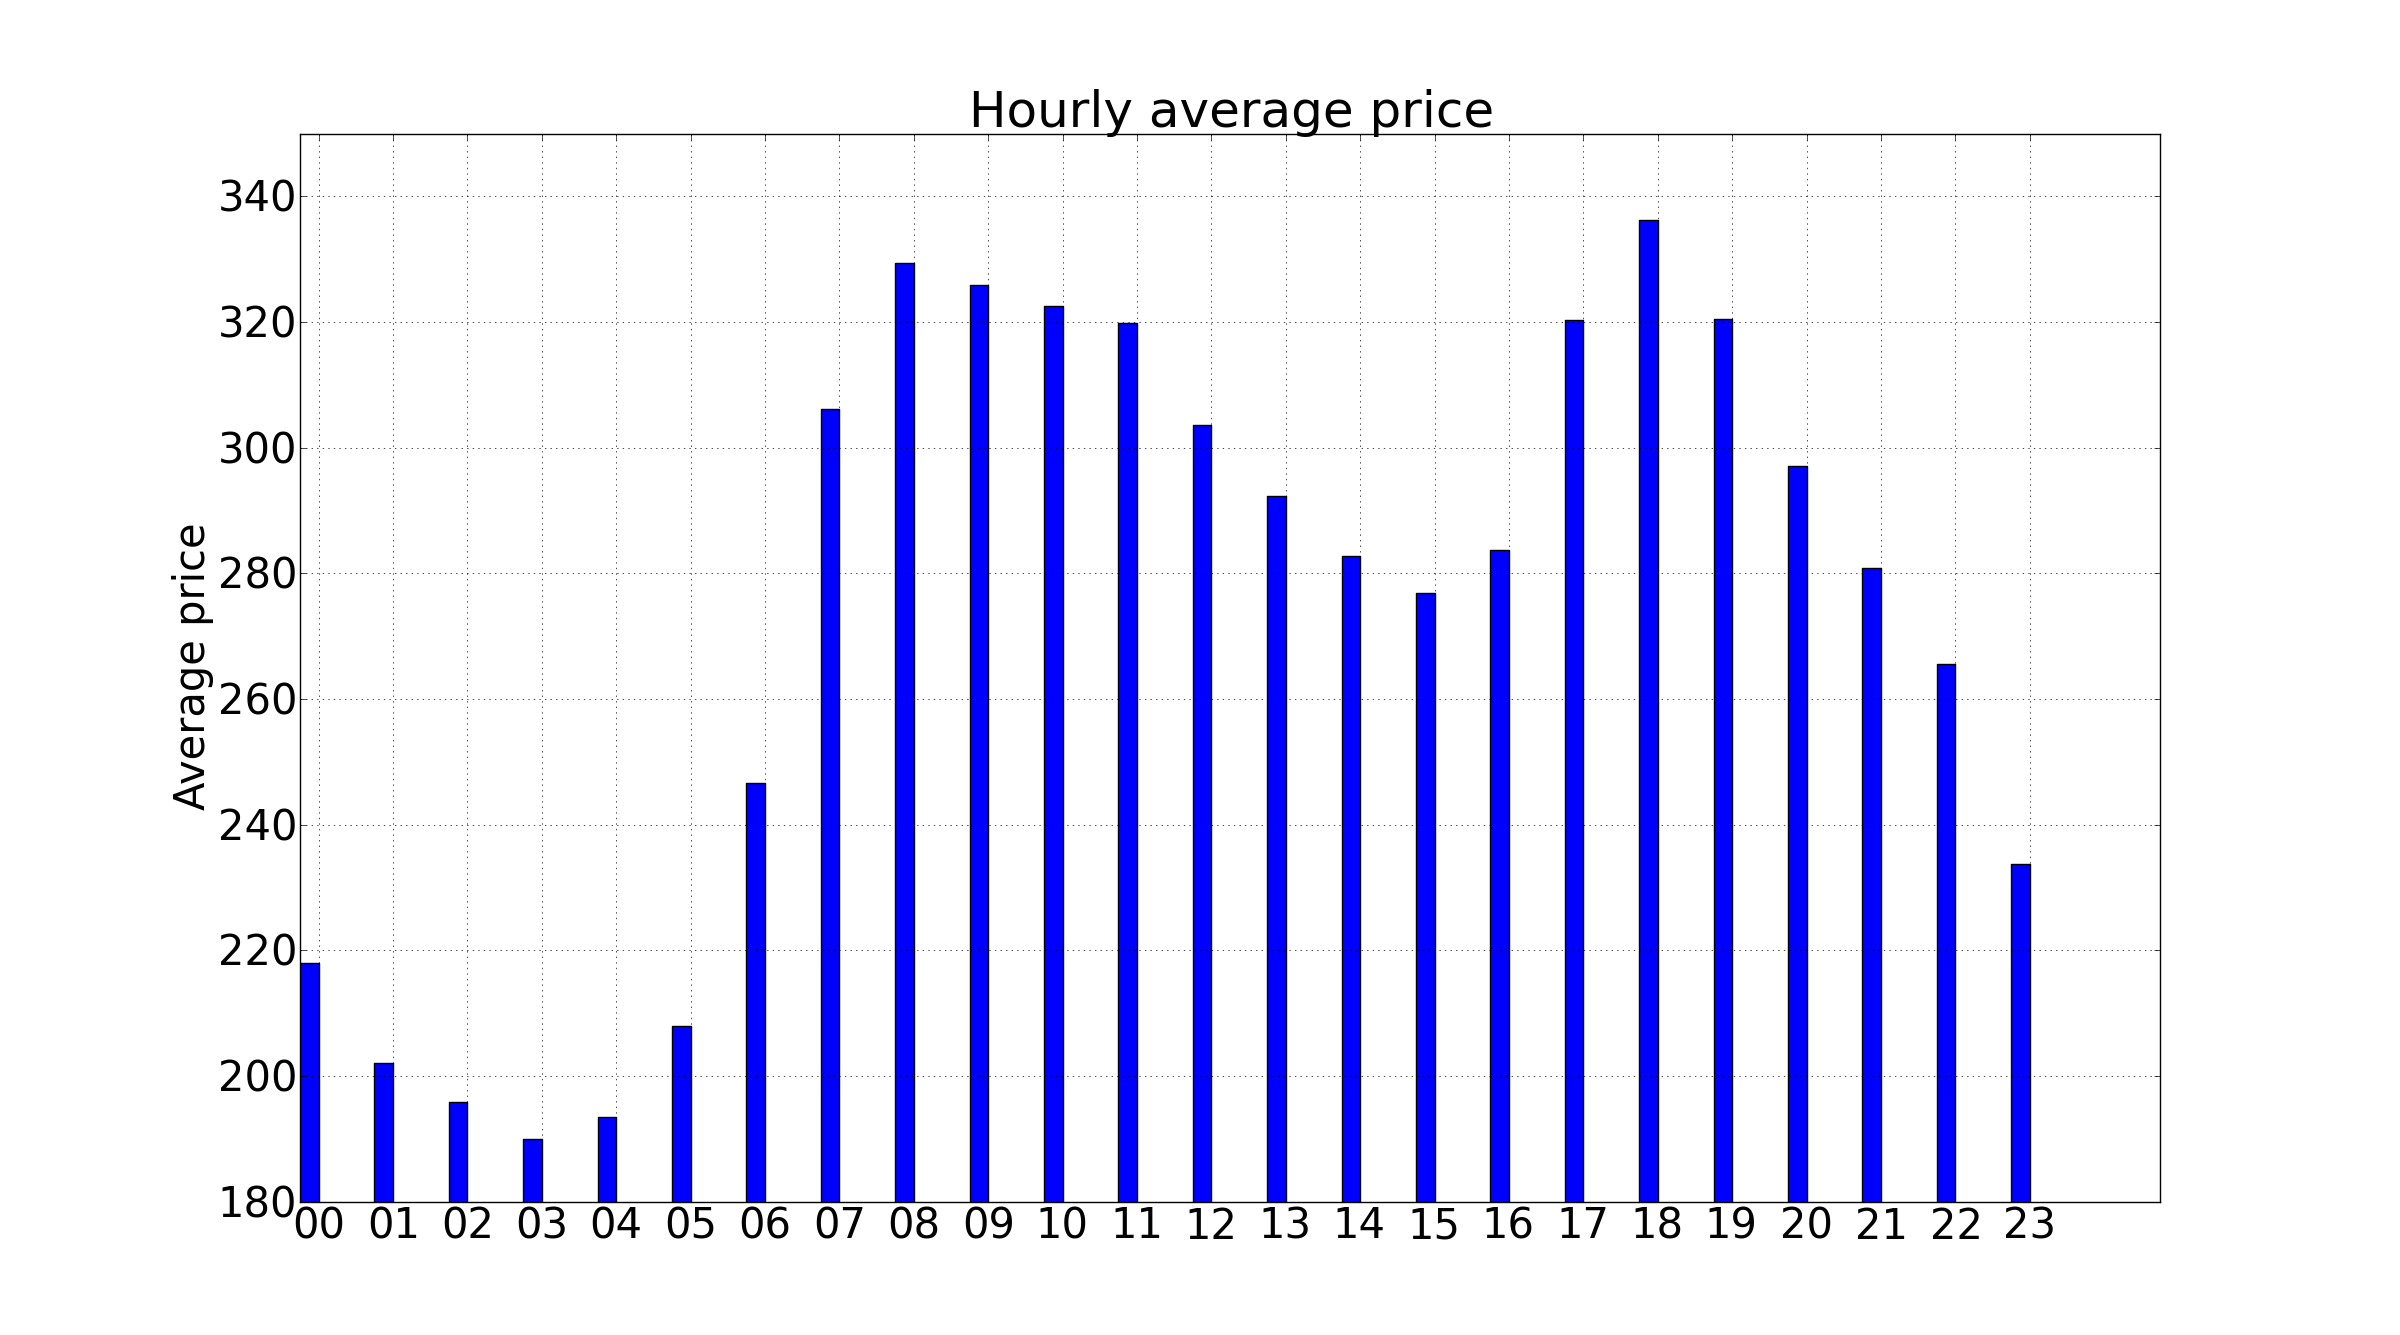
\includegraphics[width=0.8\textwidth ,natwidth=410,natheight=237]{billeder/energy_price_plots/price_per_hour.png}
\caption{}
\label{fig:price_per_hour}
\end{figure}

In ~\ref{fig:price_per_hour} we see the average price per hour over a whole day. We see a trend where the price is highest from 08 to 10 and again from 17 to 19. This is because most people wake up in the first interval and use a lot of electricity on getting ready for the day and the second interval is when everybody gets home and cooks dinner. As mentioned before we want to experiment with an ANN that is different per hour. This will require 24 networks one for each hour in a day this is because of the high fluctuation in price over all of the hours.

\begin{figure}[!ht]
\centering
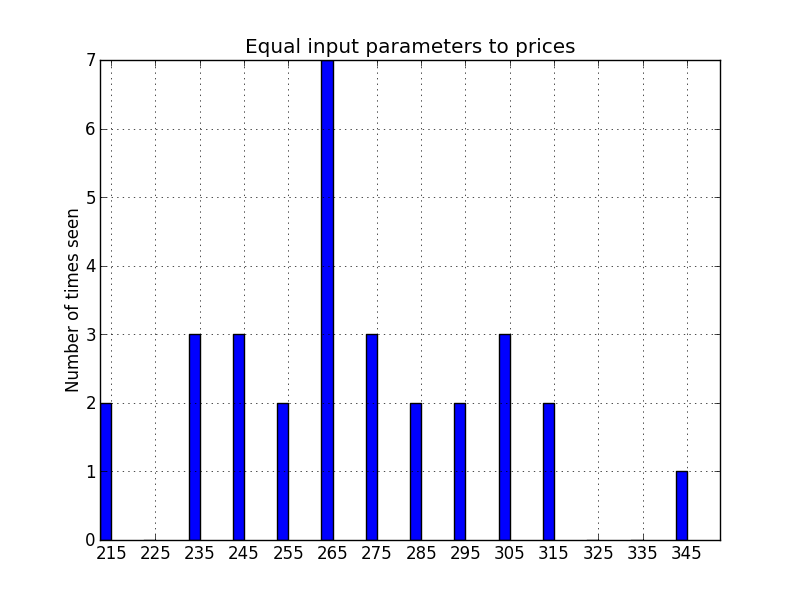
\includegraphics[width=0.8\textwidth ,natwidth=410,natheight=237]{billeder/energy_price_plots/same_hour_distribution.png}
\caption{}
\label{fig:same_hour_distribution}
\end{figure}

In the earlier figures we have shown how the input influences the price and given some reasons to why this influences the price. In figure ~\ref{fig:same_hour_distribution} we have chosen similar hours across all days of a year and we show how different the price can be for similar inputs. Even though the price is volatile we can see a trend in the graph that shows us that the price most of the time will be between 246 and 285. The hours is chosen between the limits shown in table ~\ref{table:similarHoursLimits}.

\begin{table}[!ht]
\centering  % used for centering table
\begin{tabular}{c c c c} % centered columns (3 columns)
 & \#1 Windspeed & \#2 Temperature & \#3 Demand \\ [0.5ex] % inserts table 
%heading
\hline                  % inserts single horizontal line
High margin: & 6.12 & -4.08 & 2845.8  \\
Low margin: & 5.88 & -3.92 & 2734.2 \\ [1ex] % [1ex] adds vertical space
\hline %inserts single line
\end{tabular}
\caption{This is the high and low margins for our similar hours comparison.} % title of Table
\label{table:similarHoursLimits} % is used to refer this table in the text
\end{table}


